\documentclass[CJK]{z-beamer}
\usepackage{ifthen}
\usepackage{multicol}
\usepackage{booktabs}           % toprule, bottomrule
\usepackage{tabularx}           %
    \makeatletter
    \newcommand{\thickhline}{%
        \noalign {\ifnum 0=`}\fi \hrule height 1pt
        \futurelet \reserved@a \@xhline
    }
    \newcolumntype{"}{@{\hskip\tabcolsep\vrule width 1pt\hskip\tabcolsep}}
    \makeatother
\usepackage{tikz}
    \usetikzlibrary{arrows, chains, patterns}

\usetheme{Warsaw}
\usecolortheme{spruce}

\title[信息安全与对策]
    {信息安全讲解与实施对策}
\subtitle{智恒企业信息管理系统信息安全解决方案}
\author{谢继雷}
\authorEmail{xjl@bee32.com}

\renewcommand\sectiontoc{
    \ifthenelse{\equal{\thepart}{1}}{ %
        \small
        \begin{multicols}{2} %
            \tableofcontents[currentsection,subsectionstyle=show/show/shaded]
        \end{multicols}
    }{
        \tableofcontents[currentsection,subsectionstyle=show/show/shaded]
    }
}

\begin{document}

    \begin{frame}
        \begin{center}
            \titlepage
        \end{center}
    \end{frame}

\part {信息安全讲解}

    \section {系统安全}
        \itemssframe<+->{操作系统安全}{
            \item 病毒、木马程序
            \item 溢出漏洞、Shell Code
            \item 注册表、浏览器插件
            \item 键盘钩子程序
        }
        \itemssframe<+->{公司管理安全}{
            \item 内部作案:内部员工对公司资源的非法使用
            \item 组织渗透:黑客通过利用内部员工入侵公司的网络
            \item 改进管理:自上而下的安全
            \item 技术变革:自下而上的安全
        }

    \section {通信安全}
        \itemssframe<+->{常见的通信设备和安全}{
            \item 有限通信设备
              \begin{itemize}[<+->]
                \item 集线器和交换机
                \item 路由器
                \item 带侦听端口的路由器
              \end{itemize}
            \item 无线通信设备
              \begin{itemize}[<+->]
                \item 无线路由器
                \item War-Driving、WEP、MAC-Filter
                \item 尽可能采用 WPA 加密
              \end{itemize}
            \item 防火墙
        }

        \itemssframe<+->[中间人攻击]{中间人攻击(Mitm Attack)}{
            \item 攻击采用的方法:
              \begin{itemize}[<+->]
                \item ARP 欺骗、IP 欺骗、DNS 欺骗
                \item 钓鱼网站
              \end{itemize}
            \item 攻击采用的工具:
              \begin{itemize}[<+->]
                \item SnifferPro, Wireshark,TcpDump,流光扫描软件等
                \item 黑客专用中继器、路由器、无线接入点等
              \end{itemize}
            \item 危害:
              \begin{itemize}[<+->]
                \item 重要信息泄露:登录密码、交易数据等
                \item 事务重放:重发加密的数据包
                \item 交易篡改:拦截数据包,修改之后再发送
              \end{itemize}
        }

        \subsection {传输层安全 SSL/TLS}
            \begin{frame}
                \frametitle{传输层安全 SSL/TLS}
                \begin{minipage}[c]{0.6\textwidth}
                    \begin{itemize}[<+->]
                        \item OSI 七层网络模型 \only<+->{}
                        \item HTTPS 与 SSL 的关系
                        \item 安全证书(X.509数字证书)
                        \item 支持 HTTPS 的浏览器
                    \end{itemize}
                \end{minipage}
                % \hfill
                \begin{minipage}[c]{0.3\textwidth}
                    \begin{flushright}
                    \only<1> {
                        \begin{tabular}{!{\vrule width 2pt}c|c!{\vrule width 2pt}}
                            \noalign{\hrule height 2pt}
                            应用层 & 7 \\ \hline
                            表达层 & 6 \\ \hline
                            会话层 & 5 \\ \noalign{\hrule height 1.3pt}
                            传输层 & 4 \\ \noalign{\hrule height 1.3pt}
                            网络层 & 3 \\ \hline
                            数据链路层 & 2 \\ \hline
                            物理层 & 1 \\ \noalign{\hrule height 2pt}
                        \end{tabular}
                    }
                    \only<2->{
                    \uncover<2> {
                        \begin{tikzpicture}[
                                start chain=going below,
                                node distance=5mm,
                                every node/.style={on chain, join},
                                every join/.style={->},
                                module/.style={
                                    rectangle, rounded corners=1mm,
                                    minimum size=6mm,
                                    draw=black!50
                                    %, top color=white, bottom color=black!10
                                    },
                                crypted/.style={
                                    fill=black!20,
                                    pattern=dots
                                    }
                                ]
                            \node [module] {QQ/张三};
                            \node [module] {会话层};
                            \node [module, crypted] {SSL};
                            \node [module, crypted, on chain=going below right, xshift=-3em] {网络/物理层$\cdots$};
                            \node [module, crypted, on chain=going above right, xshift=-3em] {SSL};
                            \node [module, on chain=going above] {会话层};
                            \node [module, on chain=going above] {QQ/王五};
                        \end{tikzpicture}
                    }}
                    \end{flushright}
                \end{minipage}
            \end{frame}

            \begin{frame} % \dissolve
                \frametitle{在 IE 中访问 HTTPS 的网站}
                \begin{center}
                    \raisebox{1em}{\fbox{
                      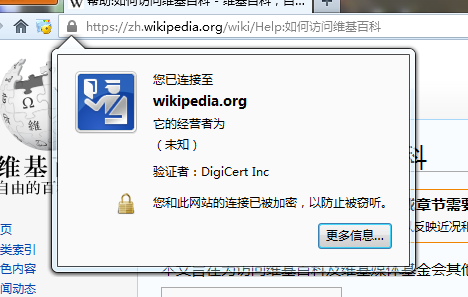
\includegraphics
                        [width=\textwidth, height=0.7\textheight]
                        {ie-https.png}
                    }}
                \end{center}
            \end{frame}

    \section {数据存储安全}

        \itemssframe<+->{数据备份}{
            \item 数据类型
              \begin{itemize}[<+->]
                \item 可变的数据
                \item 保存历史版本的数据
                \item 衍生的数据
              \end{itemize}
            \item 数据备份类型
              \begin{itemize}[<+->]
                \item 完全备份
                \item 增量备份
                \item 光盘备份/磁带备份
              \end{itemize}
        }
        \itemssframe<+->{数据冗余}{
            \item 缓存
              \begin{itemize}[<+->]
                \item 客户端缓存
                \item 前端缓存
                \item 中间层缓存
                \item 持久层缓存
              \end{itemize}
            \item RAID 冗余磁盘阵列
            \item 应用层数据冗余
        }

    \section {访问安全}

        \itemssframe<+->{访问安全和资源}{
            \item 访问安全也称为 “访问控制” 或 “用户权限设置”
            \item 高级资源:企业应用资源
            \item 低级资源:系统底层资源
            \item 资源的控制点
              \begin{itemize}[<+->]
                \item 所有
                \item 访问点:资源上的一个具体操作过程
                \item 访问点的简化分类:读、写、执行
              \end{itemize}
        }

        \itemssframe<+->{访问控制的方式}{
            \item 属主(Owner User),属组(Owner Group)
            \item 访问控制列表(ACL)
            \item 记录访问控制
            \item 事务操作访问控制
        }

        \itemssframe<+->{访问控制列表(ACL)}{
            \item ACL 的结构
              \begin{itemize}[<+->]
                \item 安全主体:用户,组,角色
                \item 有别于CRM的人员、部门、组织机构
                \item 访问控制条目(ACE):Who(谁)/What(什么资源)/How(什么权限)
              \end{itemize}

            \item 设计 ACL 的原则
              \begin{enumerate}[<+->]
                \item 用主体关系来反应企业组织
                \item 拒绝优先(Deny-First)原则
                \item 适度设计而不是过度设计
              \end{enumerate}
        }

        \itemssframe<+->{访问控制列表(ACL)的优缺点}{
            \item 优点:
              \begin{enumerate}[<+->]
                \item 可以精确地控制资源的访问
                \item 可以重用设计
                \item 可以高效实现\footnote{通过预编译技术,ACL 的匹配速度可以达到 $O(n)$。}
              \end{enumerate}

            \item 缺点:
              \begin{enumerate}[<+->]
                \item 复杂,难以使用
                \item 容易“过度安全”,导致业务过程暂停
                %\item 避免 ACE-泛化抽象废话
              \end{enumerate}
        }

        \itemssframe<+->{综合应用}{
            \item 记录访问控制
              \begin{itemize}[<+->]
                \item 记录的属主,记录过户
                \item 记录上的 ACL
                \item 记录上的默认 ACL
              \end{itemize}

            \item 事务操作访问控制
              \begin{itemize}[<+->]
                \item 事务操作的 ACL
                \item 记录上的混合操作安全
              \end{itemize}
        }

    \section {登录安全}

        \itemssframe<+->{密码安全}{
            \item 也称为“帐号安全”、“登录安全”
            \item 80\% 的系统遭到入侵是因为密码过于脆弱!
            \item 密码策略,黑客词典
            \item 与系统安全集成
        }
        \itemssframe<+->{密钥安全}{
            \item 密码的缺陷
            \item 公共密钥基础设施(PKI)
            \item 智能口令卡
            \item 密钥分发与保管
            \item 密钥过期与吊销
        }

\part {安全对策与实现}

    \section {智恒信息安全对策}
        \itemssframe<+->{信息安全规划}{
            \item 构建安全的系统 需要良好的设计
            \item 信息安全是不断完善的过程
            \item 把握安全与提供服务的关系
            \item 企业同样需要防范 信息安全的风险意识
        }
        \itemssframe<+->{智恒关于信息安全的实现}{
            \item 系统安全:采用 GNU/Linux 系统,从根本上保障系统安全
            \item 管理安全:规范数据库维护作业,只有系统管理员可以直接访问
            \item 数据安全:高可靠性服务器,RAID 阵列,增量数据库备份,文件多点镜像
            \item 访问安全:记录属主、ACL、访问点联合控制
            \item 通信安全:HTTPS 协议、安全证书分级
            \item 登录安全:密码加密存储
        }

    \section {安全实施成本}
        \itemssframe<+->{服务商方面的安全成本}{
            \item 系统安全:需要购买服务器专用的杀毒软件
            \item 管理安全:需要聘请安全专家,或交给专业ISP托管
            \item 数据安全:需要更多的存储空间
            \item 访问安全:需要更复杂的查询
            \item 通信安全:需要占用更多的计算资源
        }
        \itemssframe<+->{客户方面的安全成本}{
            \item 系统安全:需要购买桌面系统专用的杀毒软件
            \item 管理安全:需要咨询有经验的公司治理专家
            \item 数据安全:需要购买光盘、或磁带用于定期备份
            \item 访问安全:需要专业人员负责实施
            \item 登录安全:需要用户定期修改密码,或更新密钥等
            \item 通信安全:需要占用更多的计算资源
        }

\end{document}
